\documentclass[aspectratio=169,12pt]{beamer}
\usetheme{Madrid}
\usecolortheme{dolphin}
\usefonttheme{professionalfonts}
\setbeamertemplate{navigation symbols}{}
\setbeamertemplate{footline}{}

\usepackage[T1]{fontenc}
\usepackage[utf8]{inputenc}
\usepackage{graphicx}
\usepackage{amsmath,amssymb}
\usepackage{hyperref}
\usepackage{siunitx}
\usepackage{physics}
\usepackage{braket}

\graphicspath{{../../figures/}}

\title[Module B1]{Module B1: Qiskit -- module \texttt{quantum\_info}}
\author{JAMOTTE Maxime, SCHOONEN Cédric}
\institute{Digital Learning Hub}
\date{}

\begin{document}

\begin{frame}
  \titlepage
\end{frame}

\begin{frame}{Objectifs du module B1}
  \begin{itemize}
    \item Partie 1: Introduction du module \texttt{quantum\_info} et opérations sur un qubit\\~\\
    \item Partie 2: Mesures sur un qubit\\~\\
    \item Partie 3: Opérations sur deux qubits\\~\\
    \item JN = Jupyter Notebook
  \end{itemize}
\end{frame}

% ============================================================
\section{Partie 1: Introduction et opérations sur un qubit}
% ============================================================

\begin{frame}{États et portes à 1 qubit (voir JN)}
  \begin{itemize}
    \item États \(\ket{0}\) et \(\ket{1}\) construits avec \texttt{Statevector}.\\~\\
    \item Portes \(H\) et \(X\) définies avec \texttt{Operator} et appliquées via \texttt{Statevector.evolve}.\\~\\
    \item Circuits équivalents créés avec \texttt{QuantumCircuit} puis convertis en \texttt{Statevector.from\_instruction}.\\~\\
    \item Visualisation rapide des circuits avec \texttt{qc.draw('mpl')}.
  \end{itemize}
\end{frame}

\begin{frame}{Portes quantiques à un qubit (voir JN)}
  \begin{itemize}
    \item Porte de Hadamard ($H$)
    \\~\\
    \item Porte NOT ($X$)
  \end{itemize}
  \vfill
  \begin{columns}[T,onlytextwidth]
    \column{0.48\textwidth}
    \centering
    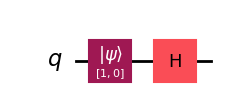
\includegraphics[width=0.8\linewidth]{gate_hadamard.png}
    \\[-0.3em]\footnotesize Circuit Qiskit pour $H$
    \column{0.48\textwidth}
    \centering
    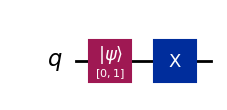
\includegraphics[width=0.8\linewidth]{gate_x.png}
    \\[-0.3em]\footnotesize Circuit Qiskit pour $X$
  \end{columns}
\end{frame}

\begin{frame}{Porte Hadamard: circuit et action (voir JN)}
  \begin{columns}[T,onlytextwidth]
    \column{0.5\textwidth}
    \centering
    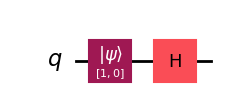
\includegraphics[width=0.75\linewidth]{gate_hadamard.png}
    \\[-0.3em]\footnotesize Circuit Qiskit pour $H$
    \column{0.5\textwidth}
    \small
    \[
      H = \frac{1}{\sqrt{2}}
      \begin{pmatrix}
        1 & 1 \\
        1 & -1
      \end{pmatrix},
      \qquad
      H\ket{0} = \tfrac{1}{\sqrt{2}}(\ket{0} + \ket{1})
    \]
    Superposition égale des deux états de base.
  \end{columns}
\end{frame}

\begin{frame}{Porte $X$ : circuit et action (voir JN)}
  \begin{columns}[T,onlytextwidth]
    \column{0.5\textwidth}
    \centering
    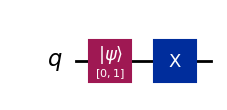
\includegraphics[width=0.75\linewidth]{gate_x.png}
    \\[-0.3em]\footnotesize Circuit Qiskit pour $X$
    \column{0.5\textwidth}
    \small
    \[
      X =
      \begin{pmatrix}
        0 & 1 \\
        1 & 0
      \end{pmatrix},
      \qquad
      X\ket{0} = \ket{1}
    \]
    Permutation des amplitudes: $|0\rangle \leftrightarrow |1\rangle$.
  \end{columns}
\end{frame}

\begin{frame}{Exercice 1 : $H$ sur \(\ket{1}\) (voir JN)}
  \begin{columns}[T,onlytextwidth]
    \column{0.55\textwidth}
    \begin{itemize}[<+->]
      \item Point de départ : \(\ket{1} = \begin{pmatrix}0\\ 1\end{pmatrix}\).\\~\\
      \item Appliquer la porte de Hadamard : \(H\ket{1} = \tfrac{1}{\sqrt{2}}(\ket{0} - \ket{1})\).\\~\\
      \item Modifier l'état initial dans le code (remplacer \(\ket{0}\) par \(\ket{1}\)) et observer la nouvelle superposition.
    \end{itemize}
    \column{0.45\textwidth}
    \centering
    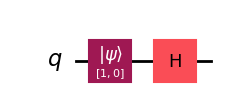
\includegraphics[width=0.8\linewidth]{gate_hadamard.png}
  \end{columns}
\end{frame}

\begin{frame}{Exercice 2 : $H$ puis $X$ sur \(\ket{0}\) (voir JN)}
  \begin{columns}[T,onlytextwidth]
    \column{0.55\textwidth}
    \begin{itemize}[<+->]
      \item Point de départ : \(\ket{0} = \begin{pmatrix}1\\ 0\end{pmatrix}\).\\~\\
      \item Chaîne d'opérations : \(X H \ket{0} = X \big(\tfrac{1}{\sqrt{2}}(\ket{0} + \ket{1})\big) = \tfrac{1}{\sqrt{2}}(\ket{0} + \ket{1})\).\\~\\
      \item Construire le circuit (H suivi de X), visualiser et vérifier l'état final dans le notebook.
    \end{itemize}
    \column{0.45\textwidth}
    \centering
    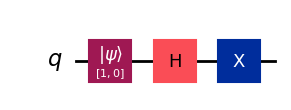
\includegraphics[width=0.8\linewidth]{gate_h_then_x.png}
  \end{columns}
\end{frame}

\begin{frame}{Exercice 3 : $X$ puis $H$ sur \(\ket{0}\) (voir JN)}
  \begin{columns}[T,onlytextwidth]
    \column{0.55\textwidth}
    \begin{itemize}[<+->]
      \item Point de départ : \(\ket{0}\).\\~\\
      \item Chaîne d'opérations : \(H X \ket{0} = H\ket{1} = \tfrac{1}{\sqrt{2}}(\ket{0} - \ket{1})\).\\~\\
      \item Comparer avec l'exercice 2 pour voir que l'ordre des portes change le résultat (non-commutativité).
    \end{itemize}
    \column{0.45\textwidth}
    \centering
    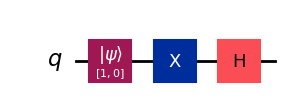
\includegraphics[width=0.8\linewidth]{gate_x_then_h.png}
  \end{columns}
\end{frame}

% ============================================================
\section{Partie 2: Mesures sur un qubit}
% ============================================================

\begin{frame}{Mesurer avec Qiskit (voir JN)}
  \begin{columns}[T,onlytextwidth]
    \column{0.5\textwidth}
    \begin{itemize}
      \item Ajouter un bit classique pour stocker la mesure: \texttt{qc(1,1)}.
      \item Opération de mesure et stockage dans le bit classique: \texttt{qc.measure(0, 0)}.
      \item Probabilités obtenues par le module carré des amplitudes: si états possibles $\ket \psi = \ket 0$, $$ P(\ket 0)=
      |\braket{0|H|\psi}|^2 = 1/2,$$  $$P(\ket 1)=|\braket{1|H|\psi}|^2 = 1/2$$
    \end{itemize}
    \column{0.45\textwidth}
    \centering
    \vspace*{-3em}
    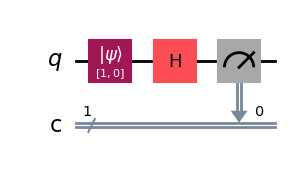
\includegraphics[width=0.9\linewidth]{measure_circuit.png}
    \\[0.05em]
    \vspace*{-1.5em}
    \[
      \begin{aligned}
        \braket{0|H|\psi} &= \begin{pmatrix} 1\\0 \end{pmatrix} \cdot \frac{1}{\sqrt 2}\begin{pmatrix} 1\\\pm 1 \end{pmatrix} = \frac{1}{\sqrt 2},\\
        \braket{1|H|\psi} &= \begin{pmatrix} 0\\1 \end{pmatrix} \cdot \frac{1}{\sqrt 2}\begin{pmatrix} 1\\\pm 1 \end{pmatrix} = \pm \frac{1}{\sqrt 2}.
      \end{aligned}
    \]
  \end{columns}
\end{frame}

\begin{frame}{La mesure projette l'état}
  \begin{columns}[T,onlytextwidth]
    \column{0.5\textwidth}
    \begin{itemize}
     \item Ajouter un bit classique et mesurer: \texttt{qc.measure(0, 0)}.
      \item Le résultat de mesure doit être stocké dans le registre classique pour être lisible.
      \item Probabilités obtenues par le module carré des amplitudes: si $\ket \psi = \ket 1$, $$ P(\ket 0)=
      |\braket{0|H|\psi}|^2 = 1/2,$$  $$P(\ket 1)=|\braket{1|H|\psi}|^2 = 1/2$$
    \end{itemize}
    \column{0.45\textwidth}
    \centering
    \vspace*{-3em}
    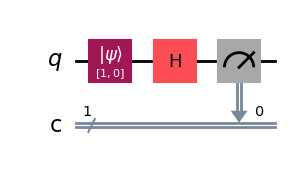
\includegraphics[width=0.9\linewidth]{measure_circuit.png}
    \\[0.05em]
    \vspace*{-1.5em}
    \[
      \begin{aligned}
        \braket{0|H|\psi} &= \begin{pmatrix} 1\\0 \end{pmatrix} \cdot \frac{1}{\sqrt 2}\begin{pmatrix} 1\\\pm 1 \end{pmatrix} = \frac{1}{\sqrt 2},\\
        \braket{1|H|\psi} &= \begin{pmatrix} 0\\1 \end{pmatrix} \cdot \frac{1}{\sqrt 2}\begin{pmatrix} 1\\\pm 1 \end{pmatrix} = \pm \frac{1}{\sqrt 2}.
      \end{aligned}
    \]
  \end{columns}
  \vspace*{-.5em}
  ~\\~\\La mesure \textbf{projette} l'état quantique sur $\ket{0}$ ou $\ket{1}$
   selon les probabilités $P(\ket 0)$ et $P(\ket 1)$. \textbf{Le système est définitivement dans un des états propres}.
\end{frame}

% ============================================================
\section{Partie 3: Opérations sur deux qubits}
% ============================================================

\begin{frame}{Opérations sur deux qubits (voir JN)}
  \begin{itemize}
    \item États à deux qubits avec \texttt{Statevector}.\\~\\
    \item Produit tensoriel et décomposition de Schmidt.\\~\\
    \item Portes à deux qubits: SWAP, CNOT, CZ.\\~\\
    \item Génération d'une paire de Bell.\\~\\
    \item Voir le Jupyter Notebook pour la pratique.
  \end{itemize}
\end{frame}

\begin{frame}{Fin du module B1}
  \centering
  \vfill
  Passons à la construction de circuits!
  \vfill
\end{frame}

\end{document}
